 \documentclass{article}

\usepackage{geometry}
\usepackage{graphicx}
\usepackage{amsmath}

\title{Interfacing HD44780U LCD display and MCS-51 based microcontroller in EDISM simulator -- an EMISY laboratory}
\author{Maciej Marcinkiewicz (300171)}
\date{29th April 2021}

\newgeometry{lmargin=3.2cm, rmargin=3.2cm, bmargin=2.5cm}

\begin{document}

\maketitle

\section{Introduction}
\subsection{Brief description}
Laboratory's main purpose was to learn the basiscs of MCS-51 (Intel 8051) assembly
programming and to learn the way of proper dealing with 2x16 Hitachi HD44780U based displays.
The task was to use 8051 microcontroller to print some characters to the LCD.

\subsection{Schematic}
\begin{figure}[h!] %possible: b, t, h, p and override (!)
    \centering
        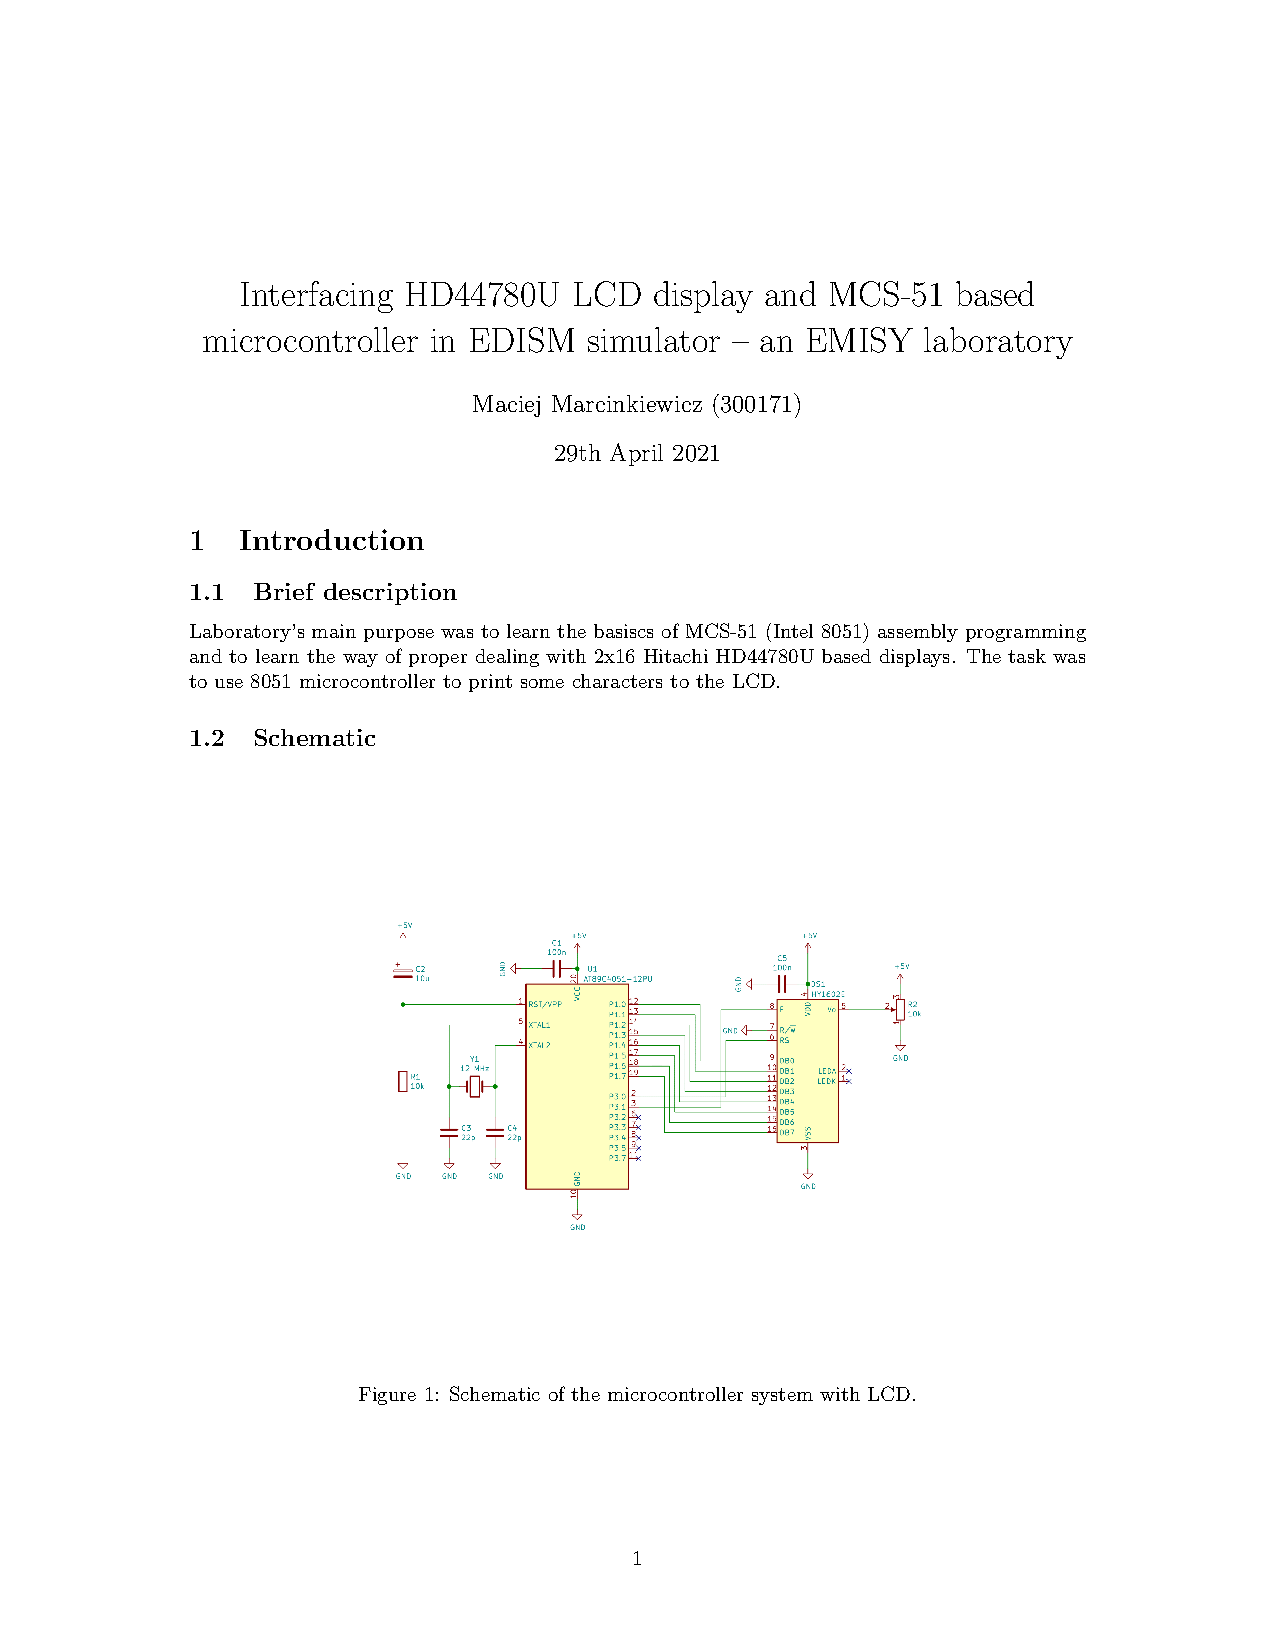
\includegraphics[width=0.9\linewidth]{schematics/lab1.png}
    \caption{Schematic of the microcontroller system with LCD.}
\end{figure}

\subsection{Hardware description}
Microcontroller (Atmel's AT89C4051) is connected to 5 V source and is equipped with 12 MHz clock and 
simple resetting circuit. LCD (HY1602E) is also connected to 5 V source. Its data bus is connected
to P1 GPIO port of the microcontroller unit. RS and E pins are connected to the P3.0 and P3.1,
respectively. LEDA and LEDK pins are not used. R/W pin is grounded, which corresponds to
permanent write (W) mode. Contrast pin V$_0$ is connected to the standard in this case 10 k$\Omega$ potentiometer.

\section{Task 1}
\subsection{Code description}
\subsubsection{8-bit mode}
Program starts with constants definition. In order to make the code more readable,
pins has been assigned to mnemonic names. Then the main routine starts with display
initialization. Assigning immiediate value to the register and decrementing it makes
a simple loop which is required for delay. In the beginning microcontroller has to wait
for display at least 30 miliseconds (in order to get proper voltage on display).
Program calls \texttt{long\textunderscore delay} subroutine 20 times in order to wait this amount of time.

\texttt{long\textunderscore delay} decrements number 256 to zero three times. It gives
appoximately 1.53 ms (even more than this). This number is not coincidence -- such delay
will be used later when several characters will be printed on display.

After 30 ms of delay data bus is filled with value responsible for function set. 
Display has to be set to two line mode. Then command is being sent by \texttt{send\textunderscore command}
subroutine. It clears RS pin as command is being sent, not data about character. In the end
it sets and then clears E pin. It is a signal for display to get data from data bus. The last
step is a short delay before the next command. \texttt{short\textunderscore delay} subroutine
is even simpler than \texttt{long\textunderscore delay}. It only decrements to zero value of 18.
It results in delay of more than 39 $\mu$s which is necessary after executing each display's command.

The next command is responsible for turning on the display and showing cursor. It is executed
in the same manner as function set. The last step in initialization process is entering
set mode. It is set to increment mode, so characters are appearing one after the other.

When initialization is finished, program is writing letter M into display's DDRAM (in the first postiton of the first line).
Letter's code is written to the data bus and \texttt{send\textunderscore data} is called.
It works almost in the same way as \texttt{send\textunderscore command}, the only difference is that
it sets R/S pin to turn on writing mode. Code is finished with an infinite loop.

\subsubsection{4-bit mode}
The task was also to perform the same operation as described previously, this time in 4-bit,
not in 8-bit mode. It means that only a half of data bus may be used. Difference is very
small -- each command and character has to be sent in two halves. For instance
instead of sending 00001110$_2$ (entry send mode) program sends firstly 0000$_2$ and then 1110$_2$.

The same applies to printing letter M. First four most significant bits are passed
(0100$_2$) and then four least significant bits (0100$_2$).

\newpage

\section{Task 2}
\subsection{Code description}
This task is performed only in 8-bit mode. Goal was to print in the first line index number
starting from 5th position of display and then to print name in the second line staring from 2nd
position. The way of writing characters is exactly the same as in task 1. The only difference is
in initial curosr placement.

To place cursor on 5th postiton in the first line command 10000100$_2$ has to be sent.
Seven least significant bits are just the address in display's memory which corresponds
to the 5th postiton (4$_{16}$). When cursor is set, program is writing characters into display's
memory. After each character writing, a longer delay is needed (more than 1.53 ms). To achive
that delay program calls \texttt{long\textunderscore delay}, which was mentioned earlier.

After printing index number, cursor has to be moved again, this time to the second line (and second position).
Its address is 41$_{16}$, so the command for setting is 11000001$_2$. The following sequence
of printing name is the same as in the case of index number. Program again ends with an infinite loop.

\section{Final questions}
\subsection*{How is 4 bit data bus configured in 2x16 LCD display?}
In order to use 4-bit mode, function set command has to be executed with 0010$_2$ in the
upper half of byte. After sending it, display ignores the lower nibble. This is why function
set is has been executed twice in the task with 4-bits -- first execution has set mode to 4-bit one.

\subsection*{Why is it convenient to use 12 MHz system clock with 8051 microcontrollers?}
It is convenient because one 8051's cycle is equal to 12 clock's oscillations. When
oscillations are of 12 MHz frequency one cycle is equal to 1$\mu$s. It makes precise
time calculations much easier.

\subsection*{Are delay methods presented in the tutorial part of the instruction optimal? Is it possible to generate precise
time intervals using loops and NOP commands?}
These methods are optimal because they allow for precise time calculation, it is possible
to adjust execution time to one 1$\mu$s as described in the previous answer. It is
also possible to use \texttt{nop} command for delay purpose, however without loops they
are sufficient only for very small delays. They could be combined with loops for longer delays
but decrementing some value in loop makes a very good delay and there is no point in using 
\texttt{nop} in such case.

\subsection*{How many 2x16 displays can you connect to the AT89C4051 microcontroller without using any additional
ICs?}
4 GPIO pins may be used as common data bus, displays may also have one common R/S pin.
Writing character occures only when E pin is set, so it is the only pin that should be
connected to the individual GPIO pin. It gives 4 + 1 common pins and 11 for E pin, thus
it is possible to connect up to 11 LCDs.

\section*{Declaration of authorship}
I declare that this piece of work which is the basis for recognition of achieving learning outcomes in the EMISY course was completed on my own.


\end{document}